Um die Frage zu beantworten wie man zwei SQL Anfragen miteinander vergleichen kann, muss man sich zunächst die Struktur einer solchen Anfrage betrachten. Exemplarisch betrachten wir im folgenden \verb|SELECT| Anfragen. Es werden mehrere Ansätze in diesem Teil der Arbeit verfolgt, wie man die Gleichheit von zwei Anfragen zeigen kann. Offensichtlich sind zwei SQL-Anfragen semantisch äquivalent, wenn sie ebenfalls syntaktisch korrekt sind. Interessanter sind daher Anfragen, die zunächst nicht syntaktisch dekungsgleich sind. 

Ein Ansatz besteht darin beide SQL-Anfragen einer Standardisierung zu unterziehen. Wie genau so etwas durchgeführt werden kann, wird im Folgenden noch erläutert. Wir würden dann zwei standardisierte SQL-Anfragen erhalten. Sind diese syntaktisch äquivalent, so handelt es sich um identische Anfragen. Dieser Ansatz wird uns mit einigen Problemen konfrontieren und daraus entwickeln wir einen zweiten Ansatz. 

Dieser versucht durch gleichartige Umformungen, die zwei Anfragen zu unifizieren (gleich zu machen). Bei diesem Ansatz würden wir also versuchen die geparsten Operatorbäume miteinander zu vergleichen. Auch diese Lösung birgt Vorteile aber auch Probleme mit sich, die im Folgenden besprochen werden.

\section{Hintergrund}

Es gibt syntaktisch unterschiedliche Anfragen, die jedoch semantisch äquivalent sind. So liefern die folgenden Anfragen die gleichen Ergebnisse, sind aber nicht syntaktisch äquivalent.

\begin{verbatim}
SELECT * FROM emp e WHERE e.enr > 5
\end{verbatim}

\begin{verbatim}
SELECT * FROM emp e WHERE 5 < e.enr
\end{verbatim}

\begin{verbatim}
SELECT * FROM emp e WHERE e.enr >= 6
\end{verbatim}

Wie man leicht sieht, sind die Anfragen ähnlich. Im folgenden werden zwei Strategien besprochen, welche beide zum Ziel haben, zwei SQL-Anfragen miteinander zu vergleichen.

\section{Standardisierung von SQL-Anfragen}

Zunächst verfolgen wir den Ansatz zwei SQL-Anfragen zu vergleichen, indem wir sie standardisieren. Die Kriterien der Standardisierung werden im Detail behandelt. Standardisiert man die Musterlösung, als auch die Lösung des Lernenden nach den gleichen Kriterien, so kann man danach durch einen einfachen Stringvergleich auf die Äquivalenz schließen. 

\subsection{Entfernen von syntaktischen Details}

Das Entfernen von syntaktischen Details übernimmt zum großen Teil bereits der Parser. Er entfernt unnötige Leerzeichen, Kommentare sowie unnötige Klammern. Aufgrund der Arbeitsweise des Parsers gibt es allerdings Situationen, in dem der Parser scheinbar nicht alle unnötigen Klammern entfernt. Wie im Abschnitt >>Verwendeter Parser<< erläutert wird, sind die geparsten Bäume nicht binär. Ein Baum wie in Abbildung \ref{baum1} zu sehen, ist daher zu vermeiden. 

Der Parser hilft allerdings dabei die SQL-Anfrage in einer Datenstruktur zu überführen, die frei von allen syntaktischen Details ist. Dazu gehören Leerzeichen, Tabs, Zeilenumbrüche und Groß/Kleinschreibung von Schlüsselwörtern.

\subsection{Vereinheitlichen der FROM Klausel}

Wir beginnen mit der Betrachtung der \verb|FROM| Klausel. Da die Reihenfolge der Spaltennamen im \verb|SELECT| Teil oft von der Aufgabenstellung vorgeschrieben ist, wird diese auch nicht verändert.

Im \verb|FROM| Teil werden zunächst alle auftretenden Tabellennamen lexikographisch sortiert. Danach werden automatische Aliase erzeugt. Sind bereits Aliase vergeben wurden, so werden diese ebenfalls durch die automatischen Aliase ersetzt. Eine Hashtabelle speichert frühere Zuweisungen, damit im \verb|SELECT| und \verb|WHERE| die Aliase ebenfalls korrekt ersetzt werden.

Hatten die vorkommenden Tabellen im \verb|FROM| Teil keinen Alias wird nur der küsntliche Alias eingeführt.

\begin{figure}
Eingabe: \\\verb|SELECT e.id, e.name, d.region FROM emp e, dep d WHERE e.depid = d.id|\\

Anpassung: \\\verb|SELECT a2.id, a2.name, a1.region FROM dep a1, emp a2 WHERE a2.depid = a1.id|\\
\caption{Beispiel: Umwandlung des FROM Teils einer SQL-Anfrage}
\end{figure}

\subsection{Umwandlung der WHERE Bedingung in KNF}

Aufgrund der Eigenheiten des ZQL-Parsers ist es möglich, dass eine unnötige Klammerung nicht entfernt wird. Beispiele dafür sind im Abschnitt >>ZQL-Parser<< zu finden. Es ist daher wünschenswert eine Normalform des \verb|WHERE| Teils zu erreichen. In diesem Fall wurde die konjunktive Normalform (KNF) gewählt.


\subsubsection{Entfernung unnötiger Klammerungen}

Ein Ausdruck \verb|((a > 5)  and ((b > 5) and (c > 5)))| enthält unnötige Klammern, da der Operator \verb|and| als Operand von einem weiteren \verb|and| vorkommt. Folgender Ausdruck ist äquivalent: \verb|((a > 5)  and (b > 5) and (c > 5))|. Diese spezielle Form der Klammerung entsteht aus der Tatsache, dass der ZQL-Parserbaum nicht binär ist und beide,  eben genannten, Beispiele nicht den gleichen Baum beschreiben. Als ersten Schritt in Richtung KNF möchten wir solchen unnötigen Klammern entfernen. 

Es ist daher wünschenswert, wenn ein Operator X einen Ausdruck als Kindknoten besitzt, in dem X ebenfalls der Operator ist, den Operator X im Kindknoten zu eliminieren und alle Kinder vom eliminierten Kindknoten an den verbleibenden Operatorknoten X zu hängen. Damit hätte man den Ausdruck vereinfacht, da die assoziative Klammerung wegfällt. Wir nennen dieses Vorgehen im Folgenden Operatorkompression.

Gegeben sei der ZQL-Parsebaum $B=(V,E)$. Es sei $child(v) = \{ w : w\in V \wedge (v,w)\in E\}$, also die Menge aller Kindknoten von $v$. Gibt es einen Knoten $w\in child(v)$ mit $v=w$, so wird Knoten $w$ eliminiert und alle Kindknoten von $w$ werden zu Kindknoten von $v$, also $child(v) = child(v) \cup child(w)$. 
$E=E\backslash \{ (w,x) : x\in child(w)\} \cup \{(v,x) x\in child(w)\}$ und $V=V\backslash \{w\}$.

Im Sinne des Vergleiches der Komplexität der Musterlösung mit der Komplexität der Lösung des Lernenden ist es sinnvoll zu speichern, ob und wie oft eine solche Operatorkompression durchgeführt werden musste.

\subsubsection{NOT auflösen}

Im nächsten Schritt möchten wir auftretende \verb|NOT| Operatoren entfernen. Dies geschieht indem der Operator \verb|NOT| im Parserbaum nach unten geschoben wird. Dabei werden die \textit{DE MORGAN} Regeln angewendet. 


Eingabe:\\
\verb|not ((a > 5)  and ((b > 5) or (c > 5)))| \\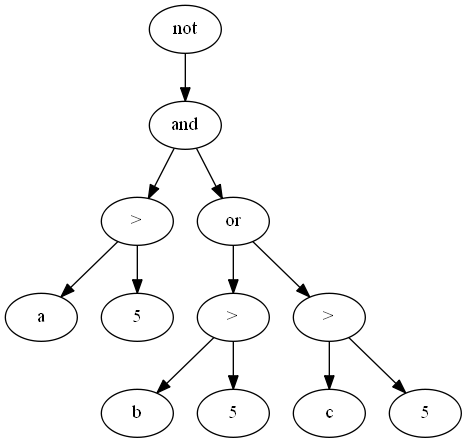
\includegraphics[scale=0.5]{Bilder/not_graph1.png}\\

Umwandlung Teil 1:\\
\verb|(not(a > 5) or not((b > 5) or (c > 5)))| \\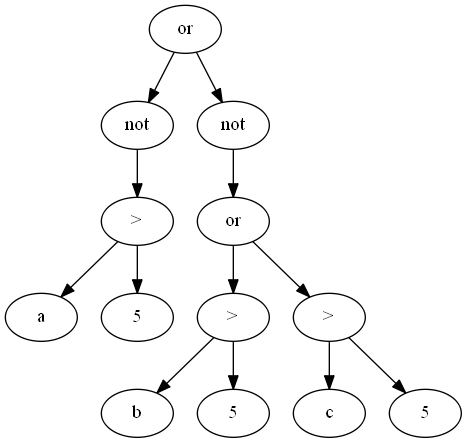
\includegraphics[scale=0.5]{Bilder/not_graph2.png}\\

\newpage
Umwandlung Teil 2:\\
\verb|((a <= 5) or (not(b > 5) and not(c > 5)))| \\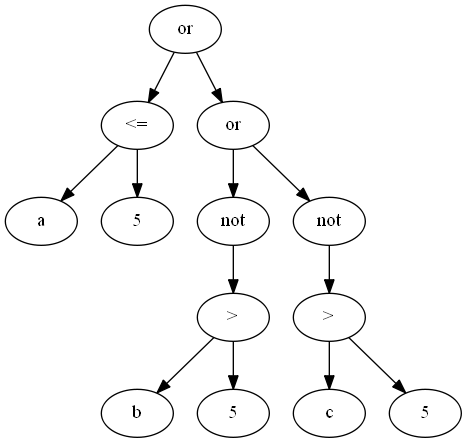
\includegraphics[scale=0.5]{Bilder/not_graph3.png}\\

Umwandlung Teil 3:\\
\verb|((a <= 5) or ((b <= 5) and (c <= 5)))| \\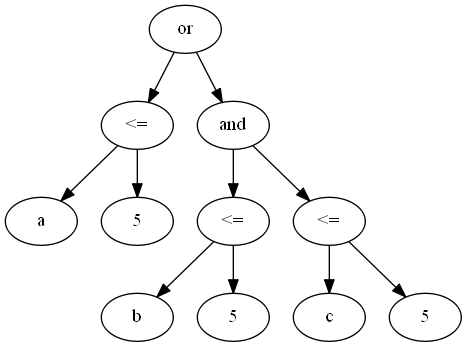
\includegraphics[scale=0.5]{Bilder/not_graph4.png}\\


\subsubsection{Anwenden des Distributivgesetzes}

Im letzten Schritt haben wir die Formel \verb|((a <= 5) or ((b <= 5) and (c <= 5)))| erhalten. Durch Anwenden des Distributivgesetzes können wir diese Formel im letzten Schritt umformen zu: \verb|((a <= 5) or (b <= 5)) and ((a <= 5) or (c <= 5))|

\subsection{Ersetzung von syntaktischen Varianten}

Um eine Anfrage zu standardisieren müssen wir den syntaktischen Zucker entfernen. Dies geschieht, in dem man nur eine syntaktische Schreibweise anerkennt und alle anderen Schreibweisen werden in die zulässige umgewandelt. Zu erwähnen sind folgende Ersetzungen, die durchgeführt werden sollen um syntaktisch vielfältige, aber semantisch äquivalente Ausdrücke zu minimieren.

\begin{figure}
\begin{tabular}{ccl}
\verb|A BETWEEN B AND C| & $\to$  & \verb|A >= B AND A <= C|\\
\verb|SELECT ALL| & $\to$ & \verb|SELECT|\\
\verb|ORDER BY VAR ASC| &  $\to$ & \verb|ORDER BY VAR|\\
\verb|EXISTS (SELECT A,B,C ...)| & $\to$ & \verb|EXISTS (SELECT 1 ...)|\\
\end{tabular}
\caption{Entfernen von syntaktischen Varianten}
\end{figure}

Ein \verb|INNER JOIN| kann sowohl im \verb|FROM|, als auch im \verb|WHERE| Teil einer SQL-Anfrage formuliert werden. Damit Untersuchungen einheitlich geschehen können, formulieren wir solche JOINs im \verb|WHERE| Teil der SQL-Anfrage.

\begin{figure}
Eingabe:\\
\verb|SELECT * FROM foo f INNER JOIN bar b ON f.id=b.id|\\

Umwandlung:\\
\verb|SELECT * FROM foo f, bar b WHERE f.id=b.id|\\
\caption{Umwandlung von INNER-JOIN}
\end{figure}

Bei Anwendung dieser Ersetzungsregeln, soll dem Lernenden ein klares Feedback gegeben werden. Es soll verdeutlicht werden, dass eine korrekte Anfrage dennoch Mängel aufweist, da unnötige Formulierungen benutzt wurden.

Eventuell ist es hier auch bereits möglich Terme, die nur aus numerischen Konstanten bestehen zu Ersetzen durch das jeweilige Ergebnisse. So könnten arithmetische Operationen bereits ausgeführt und Vergleiche, die nur aus numerischen Konstanten bestehen, durch entsprechende Wahrheitswerte ersetzt werden.

\subsection{Operatorenvielfalt}

Im folgenden Abschnitt soll geklärt werden wie mit verschiedenen Schreibweisen von ein und demselben Ausdruck umgegangen werden soll. Betrachtet man sich zum Beispiel: \verb|A > 5| ist dieser Ausdruck äquivalent mit \verb|5 < A|. Wenn wir wissen, dass \verb|A| ein ganzzahlige Variable ist, dann sind auch folgende Äquivalenzen wahr: \verb|A >= 6| so wie \verb|6 <= A|. Wir betrachten nun zwei verschiedene Ansätze um mit diesem Problem umzugehen. Ein Ansatz beschäftigt sich damit, alle implizierten Schreibweisen mit in die Formel aufzunehmen. Damit stellt man sicher, dass sich alle korrekten Schreibweisen einer Formel in der Anfrage befinden. Der zweite Ansatz beschäftigt sich damit, nur bestimmte Schreibweisen zuzulassen und alle anderen durch die zulässigen zu ersetzen.

\subsubsection{Hinzufügen implizierter Formeln}

Die Anfrage des Lernenden kann trotz zahlreicher Umformungen noch einige komplizierte Bedingungen enthalten, die wir mit bisherigen Methoden nicht entdecken konnten. Ein wichtiger Teil dabei sind transitiv-implizierte Bedingungen. Finden wir beispielsweise in der Musterlösung die Bedingung \verb|A = C AND B = C| und der Student schreibt \verb|A = B AND B = C|, so handelt es sich um semantisch äquivalente Aussagen. Damit unser Ansatz funktioniert, ist es also notwendig transitiv-implizierte Formeln immer hinzuzufügen. Wir bilden also im gewissen Sinne den transitiven Abschluss über den Operatoren $\{=,>,<\}$.

Beim Ansatz der Standardisierung mit Sortierung ist ein Betrachten von symetrischen Implikationen unnötig. Wie im Abschnitt Sortierung noch erläutert wird, werden zwei Bedingungen \verb|A = B| und \verb|B = A| nach Sortierungsregeln beide zu \verb|A = B| standardisiert. 

\subsubsection{Beschränkung der Operatorenvielfalt}

\subsection{Sortierung}

Im aktuell betrachteten Ansatz möchten wir zwei Anfragen dadurch vergleichen, dass wir sowohl die Musterlösung, als auch die Studentenlösung einer Standardisierung unterziehen. Ein ganz wesentlicher Aspekt dabei ist, die Art der Sortierung. Sind die ZQL-Parserbäume isomorph zueinander, dann lässt sich das leicht zeigen, in dem man beide nach gleichartigen Kriterien sortiert und dann einen direkten Abgleich vornimmt.

Dabei unterscheiden wir zwei Arten von Sortierung. Hat ein Operator als Operanden nur Ausdrücke und keine Konstanten oder Variablen dann sortieren wir die Kindknoten, welche jeweils wieder eigene Terme bilden.

Hat ein Operator als Operand mindestens eine Konstante oder Variable, so Sortieren wir das innere dieses Terms.

\subsubsection{Sortierung im Inneren der Terme}

Hat ein Operator \textit{OP1} als Kindknoten mindestens ein Blatt, dann werden die Kindknoten so sortiert, dass zunächst die Blattknoten (lexikographisch) und erst dann die Teilbäume erscheinen. Möglich wird dies, weil die Tabellen-Aliase in einem vorherigen Schritt bereits automatisch sortiert und benannt wurden. Bei symmetrischen Operatoren wie $=,  \textit{AND}, \textit{OR}$ können die Kindknoten einfach umgehangen/umsortiert werden. Bei Operatoren wie $\le,\ge$ ist es notwendig den Operator \textit{OP1} umzudrehen. Weil aber die Sortierung außerhalb von Termen auf den Operatoren basiert, ist es notwendig, die Sortierung im Inneren der Terme zuerst durchzuführen.

\subsubsection{Sortierung von Termen}

Hat ein Operator \textit{OP1} als Kindknoten nur weitere Operatoren \textit{OP2,OP3}, dann muss anhand dieser Operatoren die Reihenfolge im Baum festegelegt werden. Dies geschieht, in dem wir uns einfach eine Reihenfolge der Operatoren ausdenken. Wir überlegen uns folgende Ordnung $order:\textit{Relation}\to\mathbb{N}$, in der eine Relation $r$ vor einer Relation $s$ im standardisierten Parserbaum erscheint, wenn $order(r) < order(s)$.

$order:$\\

\begin{tabular}{|llllllll|}
\hline
$r\in \textit{Relation}$ & $\le$ & $\ge$ & $=$ & IS NULL & IS NOT NULL & OR & AND \\
$\textit{order}(r)$ & 1 & 2 & 3 & 4 & 5 & 6 & 7 \\
\hline
\end{tabular}\\

Es sei $\textit{RT}(\textit{OP})$ der Teilbaum des SQL-Ausdruckes mit der Wurzel \textit{OP}. Wir bezeichnen mit $\textit{depth}(\textit{RT}(\textit{OP}))$ die Tiefe des Baumes $\textit{RT}(\textit{OP})$. Es seien $\textit{child}(\textit{OP}) = \{v_1,v_2,...,v_i,...,v_n\}$ die Kindknoten von $\textit{OP}$. Die korrespondierenden Teilbäume $\textit{RT}(v_1),\textit{RT}(v_2),...,\textit{RT}(v_i),...,\textit{RT}(v_n)$ sollen nun wie folgt angeordnet werden: Der Teilbaum $\textit{RT}(v_x)$ erscheint (bei einer fiktiven BFS) vor dem Teilbaum $\textit{RT}(v_y)$ genau dann, wenn $\textit{depth}(\textit{RT}(v_x)) >  \textit{depth}(\textit{RT}(v_y))$. Die Teilbäume werden also der Tiefe nach absteigend angeordnet. 

%TODO: Gleiche Tiefe, Anordnung nach Label der Kindknoten


\section{Anpassung durch elementare Transformationen}

\section{weitere Betrachtungen}

Unabhängig von den bereits vorgestellten Ansätzen der >>Standardisierung<< und der >>Anpassung durch elementare Transformationen<< gibt es einige Umwandlungen, die entweder davor oder danach geschehen sollten. Diese Umwandlungen sollen dazu dienen dem Studenten ein Feedback zu geben. Das bedeutet, dass die Anfrage des Studenten richtig sein kann, allerdings unnötige oder unschöne Konstrukte enthält, welche die Anfrage unnötig kompliziert oder komplex machen.

Folgende verschiedene Komplexitätseinstufungen sollen eingeführt werden und auf jede Studentenanfrage angewendet werden.

\subsection{Anzahl atomarer Formeln}

Die Studentenanfrage enthält vor der Transformation durch unser Programm mehr atomare Formeln, als die Musterlösung, so wurden offensichtlich unnötige Formeln oder doppelte Formeln aufgeschrieben. Stellt unser Programm fest, dass beide Lösungen dennoch gleich sind, so muss dem Studenten mitgeteilt werden, das er redundante Formeln eingebaut hat, welche die Lösung unnötig verkomplizieren. 

\subsection{Anzahl der Operatorkompressionen}

Wie im vorherigen Abschnitt bereits erklärt ist der ZQL-Parserbaum nicht binär. Dadurch kann es durch zu vorsichtige Klammersetzung passieren, dass ein Teilbaum mit zwei Ebenen entsteht obwohl nur ein Operator beteiligt ist. Erklärt ist dies im Abschnitt >>Funktionsweise des Parsers<<. Die dort vorgestellte Operatorkompression ist ein Verfahren um unnötige Klammerungen zu entfernen. Ist die Gleichheit der Lösung des Studenten mit der Musterlösung durch unser Programm gezeigt, aber die Studentenlösung musste mehr Operatorkompressionen durchführen, so hat der Student unnötige Klammern gesetzt, welche die Lösung wiederum unnötig verkomplizieren. Dies muss ihm durch unser Programm mitgeteilt werden.

\subsection{unnötiges DISTINCT}

TODO: Algorithmus für unnötigen DISTINCT

\subsection{unnötiger JOIN}

TODO: Algorithmus für unnötigen Join

